\begin{figure*}[t]
\centering
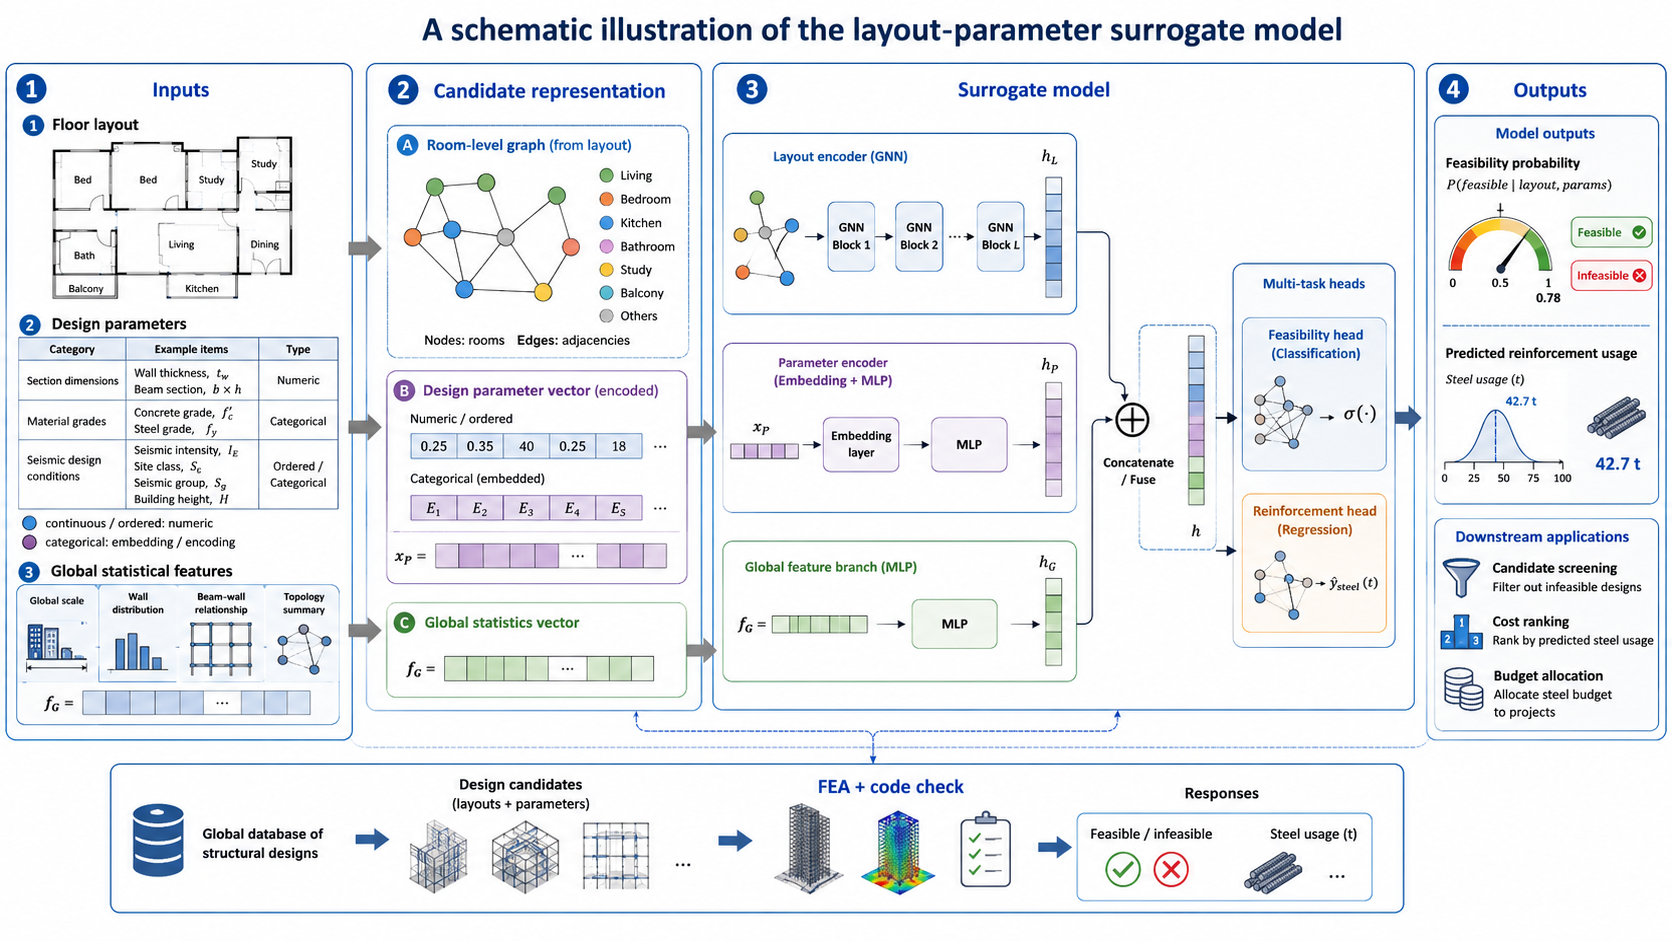
\includegraphics[width=\textwidth]{layout_parameter_surrogate.pdf}
\caption{Layout-conditioned graph surrogate model for candidate feasibility and reinforcement usage prediction.}
\label{fig:layout_parameter_surrogate}
\end{figure*}


\begin{figure*}[t]
\centering
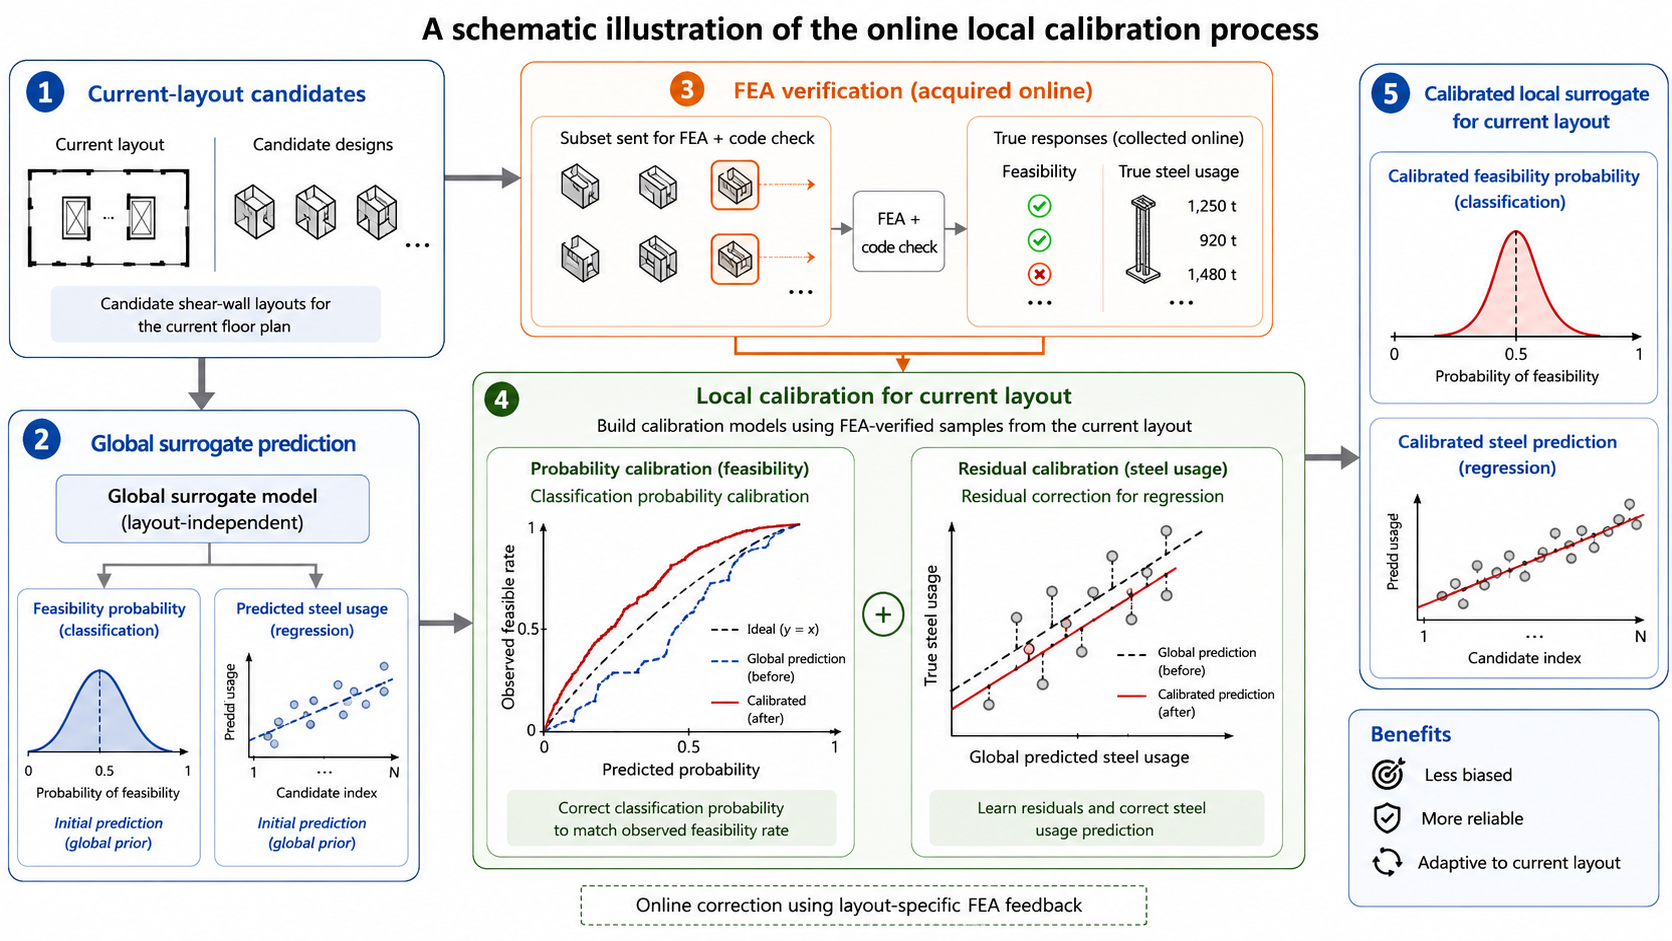
\includegraphics[width=\textwidth]{online_local_calibration.pdf}
\caption{Online local calibration of global surrogate predictions using FEA-verified samples from the current layout.}
\label{fig:online_calibration}
\end{figure*}

\begin{figure*}[t]
\centering
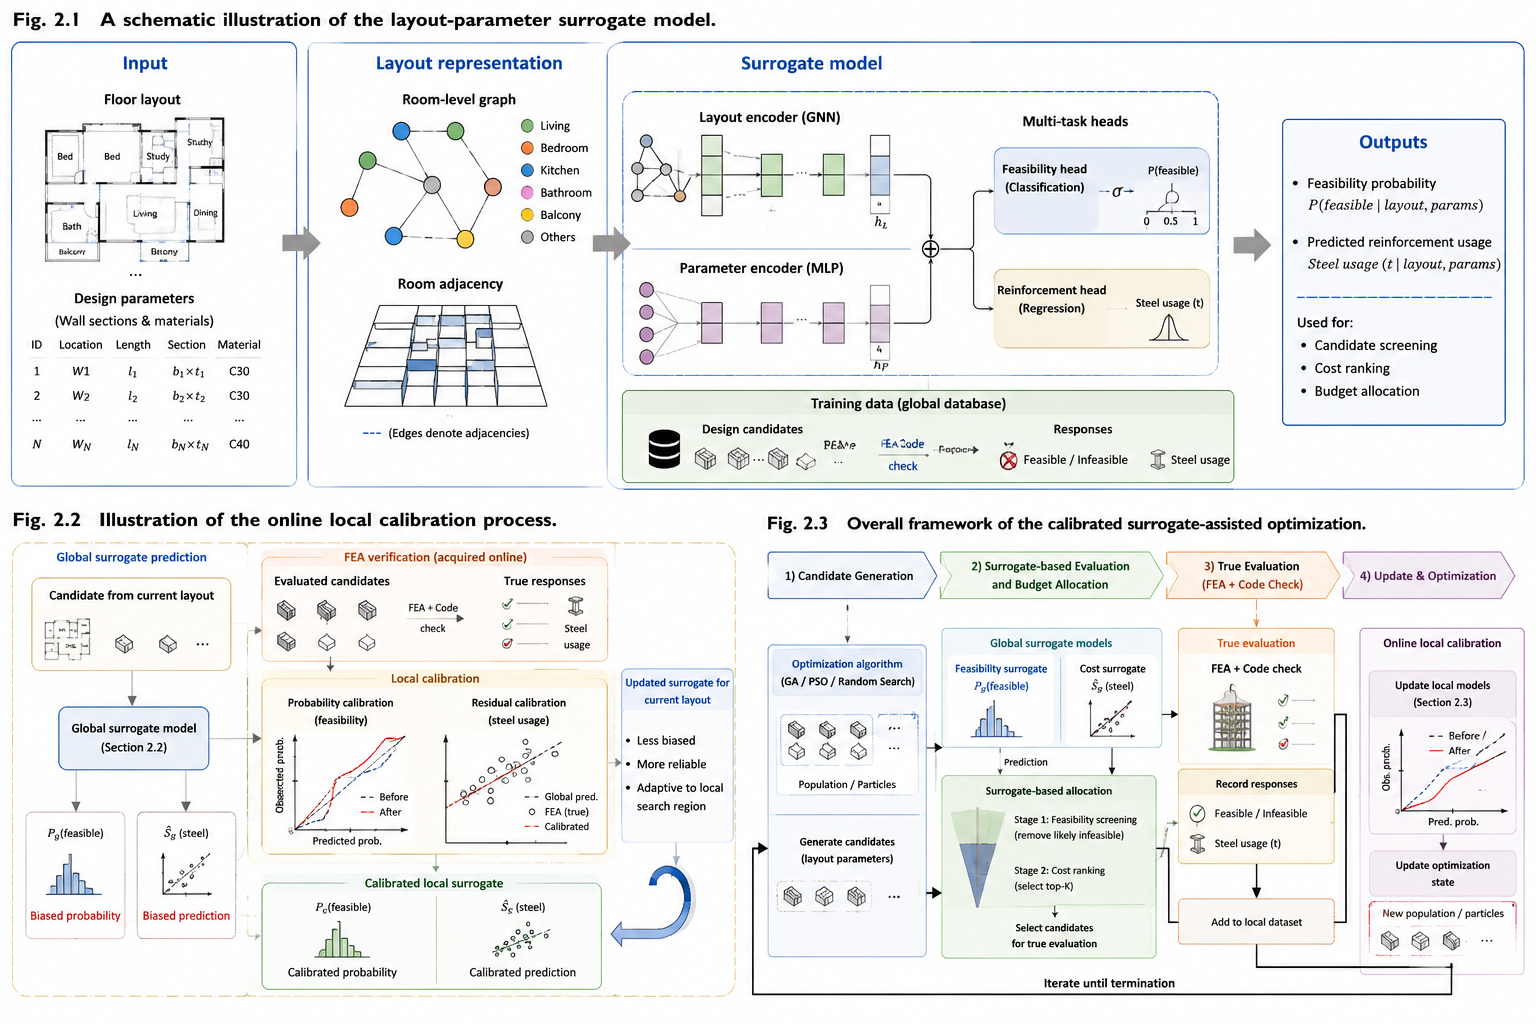
\includegraphics[width=\textwidth]{calibrated_optimization_framework.pdf}
\caption{Calibrated surrogate-assisted optimization framework.}
\label{fig:calibrated_optimization_framework}
\end{figure*}

\section{Calibrated Surrogate Modeling Method for Shear Wall Structural Optimization}
\label{sec:problem_surrogate}

To improve the efficiency of shear wall section and material optimization, the proposed method uses surrogate models to assess candidate designs before expensive FEA. In this study, true evaluation refers to the complete FEA-based workflow that generates structural responses, reinforcement design results, code-checking outcomes, and material quantities for a candidate design. A global surrogate denotes an offline model trained on FEA-verified samples from multiple layouts; it provides initial predictions of candidate feasibility and reinforcement usage. During optimization for a specific layout, candidates selected for true evaluation form a local set of newly verified samples. Online local calibration then uses this local set to correct the global surrogate predictions for the current layout. The calibrated feasibility score is used to screen clearly low-feasibility candidates, while the calibrated reinforcement prediction is used to rank promising low-cost candidates for subsequent true evaluation.

\subsection{Shear Wall Optimization Problem Formulation}
\label{subsec:expensive_problem}

For a given shear wall layout, structural optimization aims to determine suitable section and material parameters while satisfying multiple design constraints. These parameters include wall thicknesses in different vertical zones, beam section dimensions, concrete strength grades, and other design-related variables. Although the layout of the structure is fixed, different parameter combinations may lead to substantially different structural responses, reinforcement demands, and material costs.

Let $L$ denote a fixed shear wall layout and $c$ denote the corresponding design condition, including seismic intensity, site class, seismic group, load condition, and other external design requirements. The optimization variables are denoted by $x \in \mathcal{X}$, where $\mathcal{X}$ is the candidate design space formed by the allowable values of section and material parameters.

For each candidate design $(L,c,x)$, a structural evaluator $\mathcal{E}$ is required to conduct parametric modeling, FEA, structural response extraction, member design, and code-based checking\cite{GB500112010,GB500102010}. The evaluation output is written as
\begin{equation}
\mathcal{E}(L,c,x) \rightarrow (y_f,m_s,m_c,r)
\label{eq:true_evaluator}
\end{equation}
where $y_f \in \{0,1\}$ is the comprehensive feasibility label, $m_s$ and $m_c$ denote the reinforcement and concrete quantities, respectively, and $r$ represents structural response and checking indicators such as inter-story drift ratio, torsional response, axial compression ratio, shear-compression ratio, and member design results. A candidate is regarded as feasible only when the analysis is successfully completed and all major global and componet-level checks satisfy the code requirements.

The material cost of a feasible candidate is defined as
\begin{equation}
C(L,c,x)=p_s m_s(L,c,x)+p_c m_c(L,c,x)
\label{eq:material_cost}
\end{equation}
where $p_s$ and $p_c$ are the unit prices of reinforcement and concrete, respectively. In the experiments, these unit prices are determined according to current market prices. The optimization problem can therefore be formulated as
\begin{equation}
\min_{x\in\mathcal{X}} C(L,c,x),
\quad \mathrm{s.t.}\; y_f(L,c,x)=1
\label{eq:optimization_problem}
\end{equation}

The main computational difficulty lies in the repeated calls to the structural evaluator $\mathcal{E}$. In particular, reinforcement usage is difficult to estimate accurately before FEA because it depends on internal force envelopes, componet-level design, and code-based detailing requirements. Concrete quantity can be approximately obtained from geometric information and section dimensions. Therefore, this study focuses on two surrogate outputs that are most useful before FEA evaluation: (1) the probability of passing comprehensive design checks and (2) the reinforcement usage used for cost-related ranking.


\subsection{Layout-Conditioned Candidate Representation}
\label{subsec:layout_parameter_model}

The surrogate input combines layout information and design parameters. Because structural feasibility and reinforcement demand are jointly affected by the spatial layout and the design parameters, each candidate is transformed into a unified layout-conditioned representation
\begin{equation}
z=(G,d,q)
\label{eq:candidate_representation}
\end{equation}
where $G$ is the room-level graph representation of the layout, $d$ is the candidate-specific design vector formed from the design condition $c$ and the optimization variables $x$, and $q$ is the vector of global layout statistics. Thus, $z$ serves as the standard input for both surrogate tasks in this study. Fig.~\ref{fig:layout_parameter_surrogate} shows how this representation is encoded by the global surrogate models and used to predict candidate feasibility and reinforcement usage.

The first component of $z$ is the layout graph
\begin{equation}
G=(V,E)
\label{eq:layout_graph}
\end{equation}
where rooms or spatial units are treated as nodes, and adjacency relationships between rooms are treated as edges\cite{Zhao2023}. Each room node is described by a 25-dimensional feature vector that concatenates geometric descriptors and local constraint indicators. The geometric descriptors include normalized bounding-box coordinates, bounding-box size, area, and centroid, while the constraint indicators describe local buildable or wall-placement availability around the room. Each adjacency edge is assigned an 8-dimensional attribute vector that describes the spatial relationship between two neighboring rooms, including normalized shared-boundary length, shared-boundary centroid, relative direction indicators, and a boundary-orientation flag. All geometric quantities are normalized within each layout to reduce scale dependence.

The second component, $d$, encodes the seismic design condition, site information, wall and beam section parameters, concrete grade, and other candidate-level variables. The third component, $q$, supplements the graph representation with fixed-dimensional global descriptors of the whole layout. These descriptors include building scale, wall quantity, directional wall ratio, boundary wall ratio, and other geometric or topological summaries. Through this decomposition, $G$ provides local spatial organization, $q$ provides global layout context, and $d$ provides the design choices whose feasibility and cost are to be predicted.

\subsection{Global Surrogate Models and Learning Outputs}
\label{subsec:surrogate_tasks}

Given the candidate representation $z=(G,d,q)$, the global surrogate models use a layout-conditioned graph architecture to map each candidate to pre-FEA predictions. Fig.~\ref{fig:layout_parameter_surrogate}(c) shows the model architecture. The feasibility surrogate and the reinforcement surrogate are trained as two separate models with independent parameters, but they share the same input form and the same representation-learning pipeline.

The model first encodes the three components of $z$ into fixed-dimensional embeddings. The graph component $G$ is processed by a graph neural network followed by graph-level pooling, while the design vector $d$ and the global layout statistics $q$ are mapped by separate tabular encoders. The three embeddings are then concatenated into a fused candidate representation $h$. This representation is used by the separately trained feasibility and reinforcement surrogate models to produce their respective predictions.

Based on $h$, the feasibility surrogate outputs the probability that the candidate can pass the comprehensive structural checks:
\begin{equation}
\hat{p}_{f}^{G}=\sigma(f_{\theta_f}(h))
\label{eq:feasibility_output}
\end{equation}
where $\sigma(\cdot)$ is the sigmoid function and $\hat{p}_{f}^{G}\in[0,1]$. This output is used as a conservative screening score. Candidates with very low predicted feasibility can be assigned low priority, while potentially feasible candidates are retained for further ranking or true evaluation.

The reinforcement surrogate outputs the predicted reinforcement usage:
\begin{equation}
\hat{m}_{s}^{G}=f_{\theta_s}(h)
\label{eq:steel_output}
\end{equation}

This output is used as the cost-related ranking signal before FEA. Since concrete quantity can be rapidly approximated from geometry and section dimensions, the global surrogate cost estimate is written as
\begin{equation}
\hat{C}^{G}=p_s\hat{m}_{s}^{G}+p_c\tilde{m}_c
\label{eq:global_surrogate_cost}
\end{equation}
where $\tilde{m}_c$ is the estimated concrete quantity. Candidates with lower surrogate cost are assigned higher priority for true FEA evaluation after feasibility screening.

The two surrogate models are trained with task-specific losses. The feasibility model is optimized using a weighted binary cross-entropy loss to account for class imbalance:
\begin{equation}
\mathcal{L}_f = -\omega y_f \log \hat{p}_{f}^{G} - (1-y_f)\log(1-\hat{p}_{f}^{G})
\label{eq:feasibility_loss}
\end{equation}
where $\omega$ is the class weight. For reinforcement prediction, the target $m_s$ is first transformed using logarithmic scaling and standardization:
\begin{equation}
y_s=\frac{\log(1+m_s)-\mu_s}{\sigma_s}
\label{eq:steel_transform}
\end{equation}
where $\mu_s$ and $\sigma_s$ are computed from the training set. The reinforcement surrogate is trained using the Smooth L1 loss in the transformed space\cite{Huber1964}:
\begin{equation}
\mathcal{L}_s=\frac{1}{N_s}\sum_{i=1}^{N_s}\rho_\beta(e_i),
\quad e_i=\hat{y}_{s,i}-y_{s,i}
\label{eq:steel_loss}
\end{equation}
\begin{equation}
\rho_\beta(e_i)=
\begin{cases}
\dfrac{e_i^2}{2\beta}, & |e_i|<\beta, \\
|e_i|-\dfrac{\beta}{2}, & |e_i|\ge\beta
\end{cases}
\label{eq:smooth_l1}
\end{equation}
where $N_s$ is the number of reinforcement training samples and $\beta$ controls the transition between the quadratic and linear penalty regions. During inference, the predicted reinforcement usage is recovered by applying the inverse transformation of Eqn.~\ref{eq:steel_transform}.

\subsection{Online Local Calibration of Global Surrogates}
\label{subsec:online_local_calibration}

A global surrogate trained on multiple layouts provides useful prior knowledge for unseen design cases, but it may still exhibit systematic bias for a particular layout or local search region. This issue is especially important in shear wall optimization because the candidate distribution of design variable changes during the search. Therefore, using a static global surrogate throughout the optimization process may lead to inappropriate screening or ranking decisions.

To address this problem, this study introduces online local calibration. 
Fig.~\ref{fig:online_calibration} illustrates the online local calibration process.
During optimization, candidates selected for true evaluation naturally produce FEA-verified samples. These samples are accumulated as a local calibration set:
\begin{equation}
\mathcal{D}_{t}^{loc}
=
\left\{
(z_i,\hat{p}_{f,i}^{G},\hat{m}_{s,i}^{G},y_{f,i},m_{s,i})
\right\}_{i=1}^{n_t}
\label{eq:local_dataset}
\end{equation}
where $t$ denotes the current optimization iteration and $n_t$ is the number of locally verified samples. The local set stores both global surrogate predictions and true FEA-based ground truth, enabling the calibration module to learn the prediction bias of the global surrogate under the current layout.

\subsubsection{Feasibility probability calibration}
\label{subsubsec:feasibility_calibration}

For feasibility prediction, the goal of calibration is to adjust the global surrogate probability so that it better reflects the observed feasible rate in the current layout and local search region\cite{Zadrozny2002}. The global probability is first converted into a logit value:
\begin{equation}
\ell^{G}
=
\log
\frac{\hat{p}_{f}^{G}}{1-\hat{p}_{f}^{G}}
\label{eq:global_logit}
\end{equation}

When the local calibration set contains enough samples and both feasible and infeasible cases, a lightweight calibration function $g_t(\cdot)$ is fitted:
\begin{equation}
\hat{p}_{f}^{C}=g_t(\ell^{G})
\label{eq:calibrated_probability}
\end{equation}
where $\hat{p}_{f}^{C}$ is the calibrated feasibility probability.

This calibration adjusts the global feasibility probability $\hat{p}_{f}^{G}$ into a layout-specific feasibility score $\hat{p}_{f}^{C}$. The calibrated score is then used for candidate screening in the current layout. To keep the screening conservative, the threshold is chosen from locally verified feasible samples. Given a target recall $r_0$ for feasible candidates, the raw threshold is defined as
\begin{equation}
\tau_t^{raw}
=
Q_{1-r_0}
\left(
\left\{
\hat{p}_{f}^{C}\mid y_{f}=1
\right\}
\right)
\label{eq:raw_threshold}
\end{equation}
where $Q_{1-r_0}(\cdot)$ denotes the quantile function. A conservative scaling coefficient $\alpha\in(0,1]$ is then applied:
\begin{equation}
\tau_t^{C}=\alpha \tau_t^{raw}
\label{eq:calibrated_threshold}
\end{equation}

A candidate with $\hat{p}_{f}^{C}<\tau_t^{C}$ is regarded as low priority for true FEA evaluation. If there are no enough local samples for calibration, the framework falls back to the global feasibility probability and a validation-based global threshold.

\subsubsection{Reinforcement residual calibration}
\label{subsubsec:steel_calibration}

For reinforcement usage, the main purpose of calibration is to correct the systematic residual between the global surrogate prediction and the true reinforcement quantity. For a locally verified sample, the residual is defined as
\begin{equation}
\Delta m_{s}
=
m_{s}-\hat{m}_{s}^{G}
\label{eq:steel_residual}
\end{equation}

A local residual model $r_t(\cdot)$ is fitted using the local calibration set:
\begin{equation}
\widehat{\Delta m}_{s}=r_t(z,\hat{m}_{s}^{G})
\label{eq:residual_model}
\end{equation}

The calibrated reinforcement prediction is then obtained by
\begin{equation}
\hat{m}_{s}^{C}
=
\hat{m}_{s}^{G}
+
\widehat{\Delta m}_{s}
\label{eq:calibrated_steel}
\end{equation}

Compared with retraining the full graph surrogate model, this residual calibration strategy is lightweight and sample-efficient. The global surrogate captures the overall mapping learned from multiple layouts, while the local residual model only needs to correct the remaining layout-specific bias. The calibrated reinforcement prediction can be combined with the estimated concrete quantity to form a calibrated surrogate cost:
\begin{equation}
\hat{C}^{C}
=
p_s\hat{m}_{s}^{C}
+
p_c\tilde{m}_{c}
\label{eq:calibrated_cost}
\end{equation}
This calibrated cost estimate is used for candidate ranking before true evaluation.
